\documentclass[aspectratio=169,draft]{beamer}
\usepackage[utf8]{inputenc}
\usepackage[T1]{fontenc}
\usepackage{mathabx}
\usepackage{mathpazo}
\usepackage{eulervm}
\usepackage{natbib}
\usepackage{fancyhdr}
\usepackage{tikz}
\usepackage{subcaption}
\usepackage{pgfpages}
\usepackage{pifont}
\usepackage{graphicx}
\usepackage{animate}
\usepackage[dvipsnames]{xcolor}
\usepackage[most]{tcolorbox}
\usetikzlibrary{calc,shapes}
\usepackage{amssymb}

\newlength{\marginwidth}
\setlength{\marginwidth}{\paperwidth}
\addtolength{\marginwidth}{-\textwidth}

\newcommand{\tikzmark}[1]{\tikz[overlay,remember picture] \node (#1) {};}
\newcommand{\DrawBox}[1][blue!50!black]{%
    \tikz[overlay,remember picture]{
    \draw[#1]
      ($(bl)+(-0.8em,1.5em)$) rectangle
      ($(br)+(0.7em,-0.6em)$);}
}
\newcommand{\MyBox}[2][blue!50!black]{\tikzmark{bl}#2\tikzmark{br}\DrawBox[#1]}


\tikzset{
    use page relative coordinates/.style={
        shift={(current page.south west)},
        x={(current page.south east)},
        y={(current page.north west)}
    },
}

\newcommand\arcmin{\hbox{$^\prime$}}
%%%%%%%%%%%%%%%%%%%%%%%%%%%%%%%%%%%%%%%%%%%%%%%%%%


\newcommand\aap{A\&A}                % Astronomy and Astrophysics
\let\astap=\aap                          % alternative shortcut
\newcommand\aapr{A\&ARv}             % Astronomy and Astrophysics Review (the)
\newcommand\aaps{A\&AS}              % Astronomy and Astrophysics Supplement Series
\newcommand\actaa{Acta Astron.}      % Acta Astronomica
\newcommand\afz{Afz}                 % Astrofizika
\newcommand\aj{AJ}                   % Astronomical Journal (the)
\newcommand\ao{Appl. Opt.}           % Applied Optics
\let\applopt=\ao                         % alternative shortcut
\newcommand\aplett{Astrophys.~Lett.} % Astrophysics Letters
\newcommand\apj{ApJ}                 % Astrophysical Journal
\newcommand\apjl{ApJ}                % Astrophysical Journal, Letters
\let\apjlett=\apjl                       % alternative shortcut
\newcommand\apjs{ApJS}               % Astrophysical Journal, Supplement
\let\apjsupp=\apjs                       % alternative shortcut
% The following journal does not appear to exist! Disabled.
%\newcommand\apspr{Astrophys.~Space~Phys.~Res.} % Astrophysics Space Physics Research
\newcommand\apss{Ap\&SS}             % Astrophysics and Space Science
\newcommand\araa{ARA\&A}             % Annual Review of Astronomy and Astrophysics
\newcommand\arep{Astron. Rep.}       % Astronomy Reports
\newcommand\aspc{ASP Conf. Ser.}     % ASP Conference Series
\newcommand\azh{Azh}                 % Astronomicheskii Zhurnal
\newcommand\baas{BAAS}               % Bulletin of the American Astronomical Society
\newcommand\bac{Bull. Astron. Inst. Czechoslovakia} % Bulletin of the Astronomical Institutes of Czechoslovakia 
\newcommand\bain{Bull. Astron. Inst. Netherlands} % Bulletin Astronomical Institute of the Netherlands
\newcommand\caa{Chinese Astron. Astrophys.} % Chinese Astronomy and Astrophysics
\newcommand\cjaa{Chinese J.~Astron. Astrophys.} % Chinese Journal of Astronomy and Astrophysics
\newcommand\fcp{Fundamentals Cosmic Phys.}  % Fundamentals of Cosmic Physics
\newcommand\gca{Geochimica Cosmochimica Acta}   % Geochimica Cosmochimica Acta
\newcommand\grl{Geophys. Res. Lett.} % Geophysics Research Letters
\newcommand\iaucirc{IAU~Circ.}       % IAU Cirulars
\newcommand\icarus{Icarus}           % Icarus
\newcommand\japa{J.~Astrophys. Astron.} % Journal of Astrophysics and Astronomy
\newcommand\jcap{J.~Cosmology Astropart. Phys.} % Journal of Cosmology and Astroparticle Physics
\newcommand\jcp{J.~Chem.~Phys.}      % Journal of Chemical Physics
\newcommand\jgr{J.~Geophys.~Res.}    % Journal of Geophysics Research
\newcommand\jqsrt{J.~Quant. Spectrosc. Radiative Transfer} % Journal of Quantitiative Spectroscopy and Radiative Transfer
\newcommand\jrasc{J.~R.~Astron. Soc. Canada} % Journal of the RAS of Canada
\newcommand\memras{Mem.~RAS}         % Memoirs of the RAS
\newcommand\memsai{Mem. Soc. Astron. Italiana} % Memoire della Societa Astronomica Italiana
\newcommand\mnassa{MNASSA}           % Monthly Notes of the Astronomical Society of Southern Africa
\newcommand\mnras{MNRAS}             % Monthly Notices of the Royal Astronomical Society
\newcommand\na{New~Astron.}          % New Astronomy
\newcommand\nar{New~Astron.~Rev.}    % New Astronomy Review
\newcommand\nat{Nature}              % Nature
\newcommand\nphysa{Nuclear Phys.~A}  % Nuclear Physics A
\newcommand\pra{Phys. Rev.~A}        % Physical Review A: General Physics
\newcommand\prb{Phys. Rev.~B}        % Physical Review B: Solid State
\newcommand\prc{Phys. Rev.~C}        % Physical Review C
\newcommand\prd{Phys. Rev.~D}        % Physical Review D
\newcommand\pre{Phys. Rev.~E}        % Physical Review E
\newcommand\prl{Phys. Rev.~Lett.}    % Physical Review Letters
\newcommand\pasa{Publ. Astron. Soc. Australia}  % Publications of the Astronomical Society of Australia
\newcommand\pasp{PASP}               % Publications of the Astronomical Society of the Pacific
\newcommand\pasj{PASJ}               % Publications of the Astronomical Society of Japan
\newcommand\physrep{Phys.~Rep.}      % Physics Reports
\newcommand\physscr{Phys.~Scr.}      % Physica Scripta
\newcommand\planss{Planet. Space~Sci.} % Planetary Space Science
\newcommand\procspie{Proc.~SPIE}     % Proceedings of the Society of Photo-Optical Instrumentation Engineers
\newcommand\rmxaa{Rev. Mex. Astron. Astrofis.} % Revista Mexicana de Astronomia y Astrofisica
\newcommand\qjras{QJRAS}             % Quarterly Journal of the RAS
\newcommand\sci{Science}             % Science
\newcommand\skytel{Sky \& Telesc.}   % Sky and Telescope
\newcommand\solphys{Sol.~Phys.}      % Solar Physics
\newcommand\sovast{Soviet~Ast.}      % Soviet Astronomy (aka Astronomy Reports)
\newcommand\ssr{Space Sci. Rev.}     % Space Science Reviews
\newcommand\zap{Z.~Astrophys.}       % Zeitschrift fuer Astrophysik


%%%%%%%%%%%%%%%%%%%%%%%%%%%%%%%%%%%%%%%%%%%%%%%%%%%%%%%%%%%%%%%%%%



\setlength{\fboxsep}{0pt}

\newcommand\ion[2]{\text{#1\,\textsc{\lowercase{#2}}}}
\newcommand{\head}[1]{\textnormal{\textbf{#1}}}

\makeatletter
\def\sectionentry#1#2#3#4#5{% section number, section title, page
%
\newcount\mymin%
\mymin=2
\ifnum\c@section=1%
    \mymin=3
\fi%
\ifnum\c@section=2%
    \mymin=2
\fi%
%
\newcount\mymax%
\mymax=2
\ifnum\c@section=\beamer@sectionmax%
    \mymax=3
\fi%
\ifnum\c@section=\numexpr\beamer@sectionmax-1%
    \mymax=2
\fi%
%
    \ifnum\numexpr\c@section-#1<\mymax%
        \ifnum\numexpr#1-\c@section<\mymin%
            \ifnum#5=\c@part%
                \beamer@section@set@min@width
                \box\beamer@sectionbox\hskip1.875ex plus 1fill%
                \beamer@xpos=0\relax%
                \beamer@ypos=1\relax%
                \setbox\beamer@sectionbox=
                \hbox{
                    \def\insertsectionhead{#2}%
                    \def\insertsectionheadnumber{#1}%
                    \def\insertpartheadnumber{#5}%

                    {%
                        \usebeamerfont{section in head/foot}\usebeamercolor[fg]{section in head/foot}%
                        \ifnum\c@section=#1%
                            \hyperlink{Navigation#3}{{\usebeamertemplate{section in head/foot}}}%
                        \else%
                            \hyperlink{Navigation#3}{{\usebeamertemplate{section in head/foot shaded}}}%
                        \fi%    
                    }%
                }%
                \ht\beamer@sectionbox=1.875ex%
                \dp\beamer@sectionbox=0.75ex%
            \fi%
        \fi%
    \fi%
    \ignorespaces%
}

\def\slideentry#1#2#3#4#5#6{%
	%section number, subsection number, slide number, first/last frame, page number, part number
	%
	\newcount\mymin%
	\mymin=2
	\ifnum\c@section=1%
		\mymin=3
	\fi%
	\ifnum\c@section=2%
		\mymin=2
	\fi%
		%
	\newcount\mymax%
	\mymax=2
	\ifnum\c@section=\beamer@sectionmax%
		\mymax=3
	\fi%
	\ifnum\c@section=\numexpr\beamer@sectionmax-1%
		\mymax=2
	\fi%
	%
	\ifnum\numexpr\c@section-#1<\mymax%
		\ifnum\numexpr#1-\c@section<\mymin%
		  \ifnum#6=\c@part\ifnum#2>0\ifnum#3>0%
		    \ifbeamer@compress%
		      \advance\beamer@xpos by1\relax%
		    \else%
		      \beamer@xpos=#3\relax%
		      \beamer@ypos=#2\relax%
		    \fi%
		  \hbox to 0pt{%
		    \beamer@tempdim=-\beamer@vboxoffset%
		    \advance\beamer@tempdim by-\beamer@boxsize%
		    \multiply\beamer@tempdim by\beamer@ypos%
		    \advance\beamer@tempdim by -.05cm%
		    \raise\beamer@tempdim\hbox{%
		      \beamer@tempdim=\beamer@boxsize%
		      \multiply\beamer@tempdim by\beamer@xpos%
		      \advance\beamer@tempdim by -\beamer@boxsize%
		      \advance\beamer@tempdim by 1pt%
		      \kern\beamer@tempdim
		      \global\beamer@section@min@dim\beamer@tempdim
		      \hbox{\beamer@link(#4){%
		          \usebeamerfont{mini frame}%
		          \ifnum\c@section=#1%
		            \ifnum\c@subsection=#2%
		              \usebeamercolor[fg]{mini frame}%
		              \ifnum\c@subsectionslide=#3%
		                \usebeamertemplate{mini frame}%\beamer@minislidehilight%
		              \else%
		                \usebeamertemplate{mini frame in current subsection}%\beamer@minisliderowhilight%
		              \fi%
		            \else%
		              \usebeamercolor{mini frame}%
		              %\color{fg!50!bg}%
		              \usebeamertemplate{mini frame in other subsection}%\beamer@minislide%
		            \fi%
		          \else%
		            \usebeamercolor{mini frame}%
		            %\color{fg!50!bg}%
		            \usebeamertemplate{mini frame in other subsection}%\beamer@minislide%
		          \fi%
		        }}}\hskip-10cm plus 1fil%
		  }\fi\fi%
		  \else%
		  \fakeslideentry{#1}{#2}{#3}{#4}{#5}{#6}%
		 \fi%
		\fi%
	\fi%
	\ignorespaces%
}
\makeatother




\setbeamertemplate{caption}[numbered]
\setbeamerfont{caption}{size=\scriptsize}
% \setbeamercovered{transparent}
\setbeamercovered{invisible}


\usetheme{Dresden}
\usefonttheme{serif}
\usecolortheme{rose}



\setbeamertemplate{headline}{%
\leavevmode%
  \hbox{%
    \begin{beamercolorbox}[wd=\paperwidth,ht=3.5ex,dp=2.75ex]{palette tertiary}%
    \scriptsize{\insertnavigation{\paperwidth}}
    \end{beamercolorbox}%
  }
  \hbox{%
    \begin{beamercolorbox}[wd=\paperwidth,ht=0.5ex,dp=1ex]{palette secondary}%
    \end{beamercolorbox}%
  }
}

\setbeamertemplate{footline}{%
\leavevmode%
    \hbox{%
    \begin{beamercolorbox}[wd=\paperwidth,ht=0.1ex,dp=1ex]{palette secondary}%
    \end{beamercolorbox}%
  }
  \hbox{%
    \begin{beamercolorbox}[wd=\paperwidth,ht=2.5ex,dp=1ex]{palette tertiary}%
     \hspace{2.5mm} \inserttitle \hfill{} \textbf{\insertframenumber} \hspace{2.5mm}
    \end{beamercolorbox}%
  } 
}



\author[Sameer Patidar]{\vspace*{-2mm}\Large{Mid-Term 2}\\
\vspace*{7mm}
\large{Sameer Patidar}
\\ 
\vspace*{0.5mm}
SC19B161} % (optional, for multiple authors)
% {A.~B.~Arthur\inst{1} \and J.~Doe\inst{2}}

\institute[Indian Institute of Space Science and Technology] % (optional)
{
  \large{Dual Degree (Astronomy \& Astrophysics)} \\\\
\vspace{1mm}
  \large{Indian Institute of Space Science and Technology} \\\\
\vspace{5mm}
\large{Supervisors : Dr. Vikram Khaire and Dr. Anand Narayanan}
}
\logo{\includegraphics[height=1cm]{IIST.png}}

\begin{document}

% TITLE OF THE PRESENTATION

\newcommand{\titleofpresentation}{Tracing Baryons in the Warm Hot Intergalactic Medium using Broad Lyman-$\alpha$ Absorbers}

\date{\large{}}
\title{\LARGE{\textbf{\titleofpresentation}} \vspace{-3mm}}

\setbeamertemplate{headline}{%
\leavevmode%
  \hbox{%
    \begin{beamercolorbox}[wd=\paperwidth,ht=3.5ex,dp=2.75ex]{palette tertiary}%
    \end{beamercolorbox}%
  }
  \hbox{%
    \begin{beamercolorbox}[wd=\paperwidth,ht=0.5ex,dp=1ex]{palette secondary}%
    \end{beamercolorbox}%
  }
}

\setbeamertemplate{footline}{%
\leavevmode%
    \hbox{%
    \begin{beamercolorbox}[wd=\paperwidth,ht=0.1ex,dp=1ex]{palette secondary}%
    \end{beamercolorbox}%
  }
  \hbox{%
    \begin{beamercolorbox}[wd=\paperwidth,ht=2.5ex,dp=1ex]{palette tertiary}%
    \end{beamercolorbox}%
  }
  
}

\begin{frame}
\vspace*{-3mm}
\maketitle
\end{frame}

\setbeamertemplate{footline}{%
\leavevmode%
    \hbox{%
    \begin{beamercolorbox}[wd=\paperwidth,ht=0.1ex,dp=1ex]{palette secondary}%
    \end{beamercolorbox}%
  }
  \hbox{%
    \begin{beamercolorbox}[wd=\paperwidth,ht=2.5ex,dp=1ex]{palette tertiary}%
     \hspace{2.5mm} \textbf{\titleofpresentation} \hfill{} \textbf{\insertframenumber} \hspace{2.5mm}
    \end{beamercolorbox}%
  } 
}


\logo{}

% \begin{frame}
% \frametitle{\huge{{\textbf{Outline}}}}
% \tableofcontents
% \end{frame}

\setbeamertemplate{headline}{%
\leavevmode%
  \hbox{%
    \begin{beamercolorbox}[wd=\paperwidth,ht=3.5ex,dp=2.75ex]{palette tertiary}%
    \scriptsize{\textbf{\insertnavigation{\paperwidth}}}
    \end{beamercolorbox}%
  }
  \hbox{%
    \begin{beamercolorbox}[wd=\paperwidth,ht=0.5ex,dp=1ex]{palette secondary}%
    \end{beamercolorbox}%
  }
}

\setbeamertemplate{footline}{%
\leavevmode%
    \hbox{%
    \begin{beamercolorbox}[wd=\paperwidth,ht=0.1ex,dp=1ex]{palette secondary}%
    \end{beamercolorbox}%
  }
  \hbox{%
    \begin{beamercolorbox}[wd=\paperwidth,ht=2.5ex,dp=1ex]{palette tertiary}%
     \hspace{2.5mm} \textbf{\titleofpresentation} \hfill{} \textbf{\insertframenumber} \hspace{2.5mm}
    \end{beamercolorbox}%
  } 
}


\section{Thesis Phase I : Recap}

\vspace*{2.7cm}

{\huge{\textbf{Thesis Phase I : Recap}}}

\end{frame}

\begin{frame}{\huge{{\textbf{Recap}}}}

\begin{columns}
  % Consolas, 'Courier New', monospace,
    \begin{column}{0.6\textwidth} 
        \vspace{-13mm}
        \uncover<1->{
          \begin{itemize}
              \item The missing baryon problem
              \item BLAs : Way to probe WHIM
              \item Absorber towards PG 0003+158
              \item BLA survey  
        \end{itemize}
        }
    \end{column}      

    \begin{column}{0.4\textwidth}
        \uncover<4->{\begin{figure}[!htbp]
          \centering
          \includegraphics[width=5cm]{Figures/Mid-term/Baryon_distribution.png}
          \vspace*{-1mm}
          \caption{Baryon budget at $z \sim 0$. \\\\ Shull et al. (2012)}
          \label{}
        \end{figure}}
    \end{column}

\end{columns}


% sdjfsdkjf

\begin{tikzpicture}[remember picture, overlay,use page relative coordinates]
  
    \uncover<2->{\node at (0.25,0.20) {Ref. : Fukugita et al. (1998)} ;} 
    \uncover<4->{\node at (0.263,0.15) {Shull et al. (2012)} ;}
    
\end{tikzpicture}

\end{frame}
  



\begin{frame}{\huge{{\textbf{How to detect WHIM ?}}}}

\begin{columns}
    \begin{column}{0.35\textwidth} 
        \vspace{-13mm}
        \uncover<1->{
         \begin{itemize}
            \uncover<2->{\item Quasars as backlight}   
                \begin{itemize}
                \uncover<4->{\item[-] \ion{O}{vi-viii}, \ \ion{Ne}{ix-x}, \ \ion{N}{vii}, etc.}
                \uncover<5->{\item[-] \textbf{BLAs}}
                \end{itemize} 
          \end{itemize}
        }
    \end{column}
    \begin{column}{0.65\textwidth}
        \uncover<3->{
        \begin{figure}[!htbp]
          \centering
          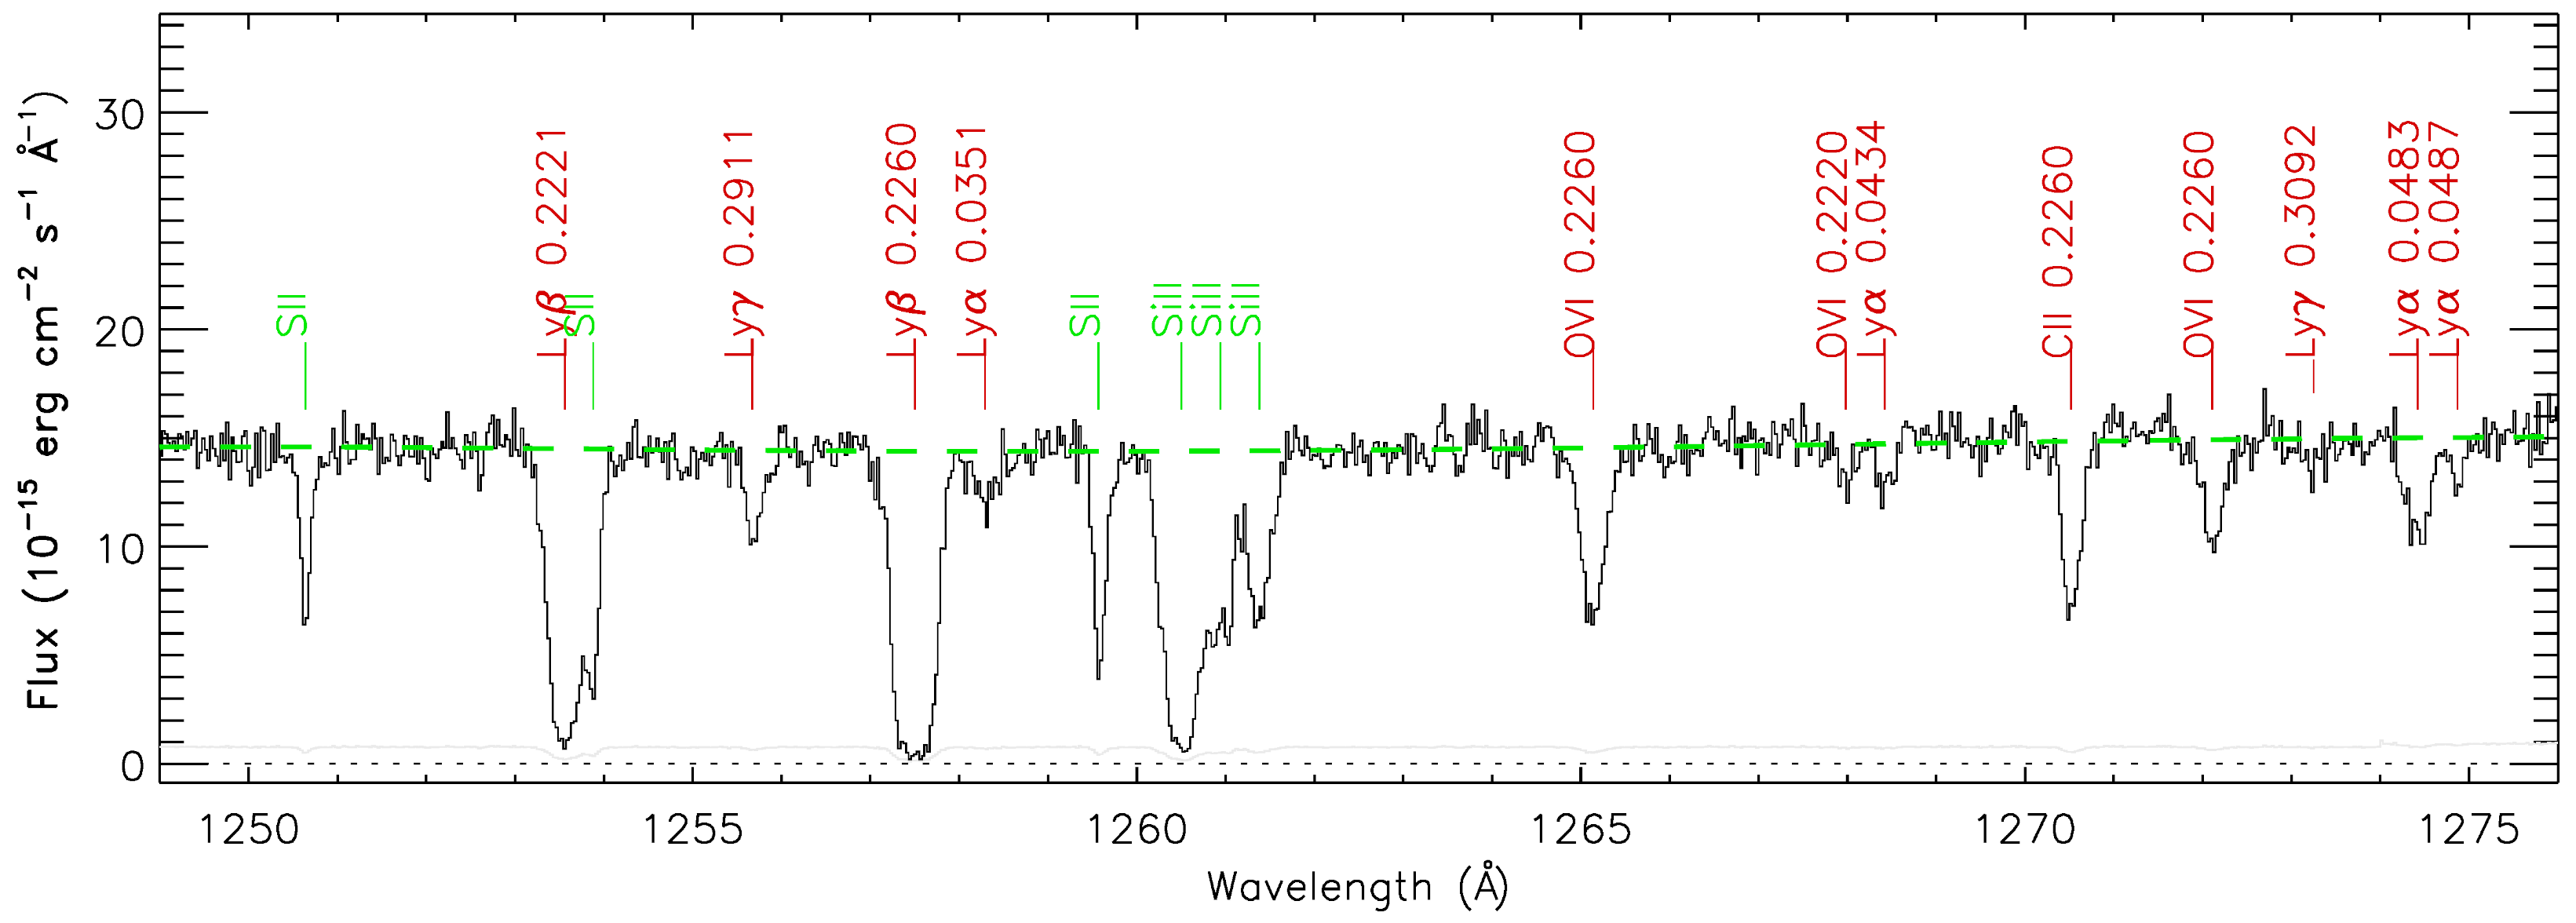
\includegraphics[width=9cm]{Figures/Mid-term/spec slice.png}
          \vspace*{-1mm}
          \caption{Slice of spectrum of quasar HE0153-4520 ($z_{em}=0.4510$). \\ Danforth et al. (2016)}
        \end{figure}}
    \end{column}
\end{columns}


\begin{tikzpicture}[remember picture, overlay,use page relative coordinates]
  
   \uncover<4->{\node at (0.20,0.17) {Ref. : Tepper-García et al. (2013)} ;
   \node at (0.20,0.12) {Savage et al. (2014)} ;}
   
\end{tikzpicture}


\end{frame}


\begin{frame}[noframenumbering]{\huge{{\textbf{How to detect WHIM ?}}}}

\begin{columns}
    \begin{column}{0.35\textwidth} 
        \vspace{-13mm}
         \begin{itemize}
            \item Quasars as backlight  
                \begin{itemize}
                    \item[-] \ion{O}{vi-viii}, \ \ion{Ne}{ix-x}, \ \ion{N}{vii}, etc.
                    \item[-] \textbf{BLAs}
                \end{itemize} 
          \end{itemize}
    \end{column}
    \begin{column}{0.65\textwidth}
        \uncover<1->{
        \begin{figure}[!htbp]
          \centering
          \includegraphics[width=9cm]{Figures/Mid-term/BLA-individual.png}
          \vspace*{-1mm}
          \caption{A BLA towards the LOS of quasar H 1821+643 $(z_{em} = 0.297)$ \\\\ Philipp Richter (2005)}
        \end{figure}}
    \end{column}
\end{columns}

\begin{tikzpicture}[remember picture, overlay,use page relative coordinates]
  
   \uncover<1->{\node at (0.20,0.17) {Ref. : Tepper-García et al. (2013)} ;
   \node at (0.20,0.12) {Savage et al. (2014)} ;}
   
\end{tikzpicture}

\end{frame}

\begin{frame}[noframenumbering]{\huge{{\textbf{How to detect WHIM ?}}}}

\begin{columns}
    \begin{column}{0.35\textwidth} 
        \vspace{-13mm}
         \begin{itemize}
            \item Quasars as backlight  
                \begin{itemize}
                    \item[-] \ion{O}{vi-viii}, \ \ion{Ne}{ix-x}, \ \ion{N}{vii}, etc.
                    \item[-] \textbf{BLAs}
                \end{itemize} 
          \end{itemize}
    \end{column}
    \begin{column}{0.65\textwidth}
        \uncover<1->{
        \begin{figure}[!htbp]
          \centering
          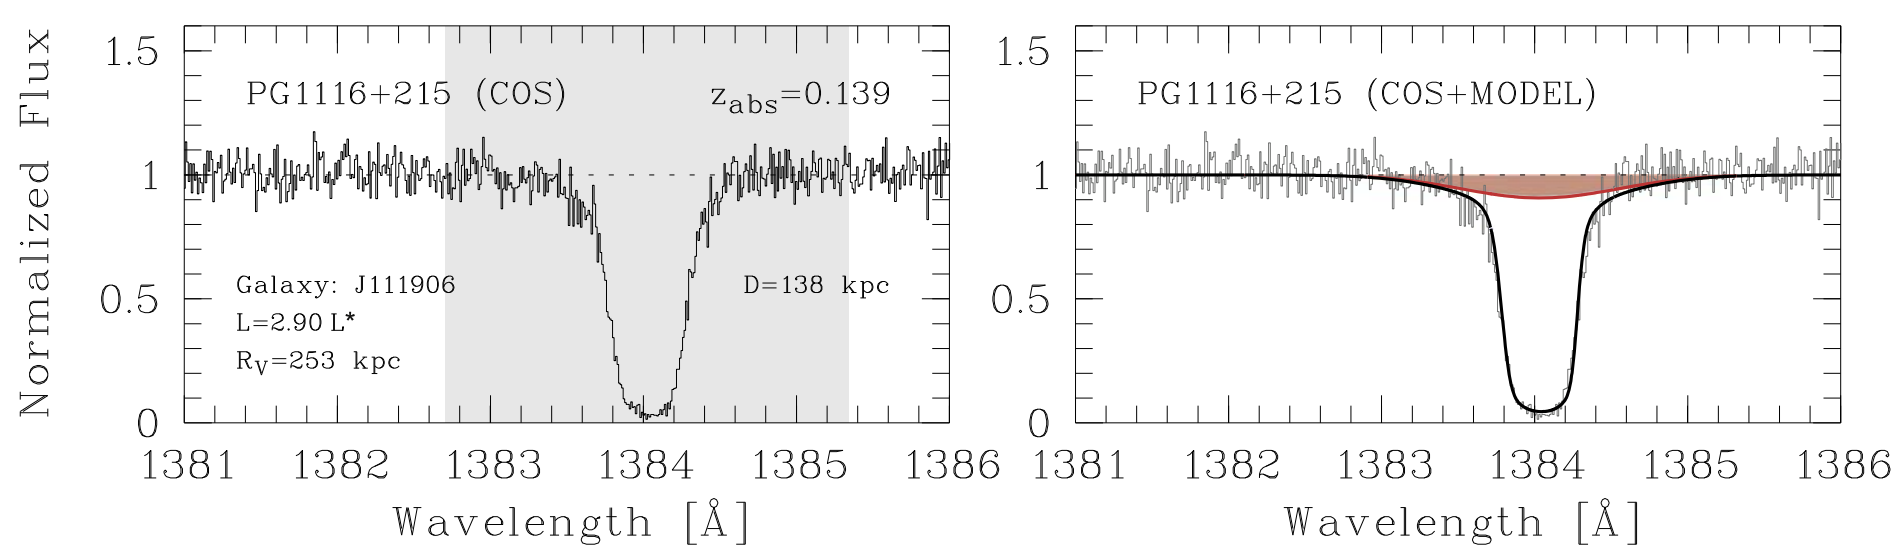
\includegraphics[width=9cm]{Figures/Mid-term/BLA.png}
          \vspace*{-1mm}
          \caption{A BLA blended with other Ly$\alpha$ absorption lines towards the LOS of quasar PG1116+215 $(z_{em} = 0.176)$. Philipp Richter (2020)}
        \end{figure}}
    \end{column}
\end{columns}

\begin{tikzpicture}[remember picture, overlay,use page relative coordinates]
  
   \uncover<1->{\node at (0.20,0.17) {Ref. : Tepper-García et al. (2013)} ;
   \node at (0.20,0.12) {Savage et al. (2014)} ;}
   
\end{tikzpicture}
    
\end{frame}


\section{Data}

\vspace*{2.7cm}

{\huge{\textbf{Data}}}

\end{frame}

\begin{frame}{\huge{{\textbf{\textit{HST}/COS Data}}}}

\uncover<1->{\begin{itemize}
    \uncover<2->{\item 82 UV-bright AGNs chosen by Danforth et al. (2016)
    \uncover<3->{\item $z_{AGN} < 0.85$}}
    \uncover<4->{\item High S/N $\gtrsim$ 15}
    \uncover<5->{\item FUV channel : G130M and G160M gratings
    \uncover<6->{\item Coverage : 1130-1790 \AA}}
    \uncover<7->{\item $\text{R} \sim 17,000 \ \approx$ 17 km $\text{s}^{-1}$} 
\end{itemize}}

\end{frame}


\section{Phase I}

\begin{frame}{}

{\huge{\textbf{Phase I}}}

\end{frame}


\section{Absorber system towards PG0003+158}


% \subsection{djdbkjdbv}

\begin{frame}{}

{\huge{\textbf{Absorber system towards PG0003+158}}}

\end{frame}


\begin{frame}{\huge{{\textbf{Absorber system}}}}

\begin{itemize}
    \item Quasar at $z_{em}=0.45089$
    \item $z_{abs} \sim$ 0.347
    \item 3 component system
\end{itemize}

\begin{figure}[!htbp]
      \centering
      \includegraphics[width=7cm]{Figures/Mid-term/Component_structure2.png}
\end{figure}

\end{frame}

\begin{frame}{\huge{{\textbf{Voigt profile fitting}}}}

\end{frame}


\begin{frame}[plain,noframenumbering]{}

\begin{figure}[!htbp]
          \centering
          \includegraphics[width=12cm]{Figures/Mid-term/PG0003+158-z=0.347579-sys-plot.png}
          \vspace*{-1mm}
          \caption{System plot of the absorber system. Velocity is taken zero at z = 0.347579}
\end{figure}   

\end{frame}


\begin{frame}{\huge{{\textbf{Voigt profile fitting}}}}

\begin{columns}
    \begin{column}{0.4\textwidth} 
        \vspace{-10mm}
         \begin{itemize}
            \item \ion{H}{i} : 3 components  
            \item \ion{O}{vi} : 2 components
            \item \ion{C}{ii}, \ion{C}{iii}, \ion{Si}{ii}, \ion{Si}{iii}  : 1 component
          \end{itemize}
    \end{column}
    \begin{column}{0.6\textwidth}
        \vspace{-3mm}
        \begin{figure}[!htbp]
          \centering
          \includegraphics[width=8cm]{Figures/Mid-term/param.png}
        \end{figure}
    \end{column}
\end{columns}

\end{frame}


\begin{frame}[noframenumbering]{\textbf{CLOUDY}}
    
\begin{figure}[!htbp]
          \centering
          \includegraphics[width=12cm]{Figures/Mid-term/cloudy-transparent.png}
          \vspace*{-1mm}
          \caption{Schematic diagram of CLOUDY simulations.}
\end{figure}
        
\end{frame}



\begin{frame}{\huge{{\textbf{Ionization Modelling}}}}

\begin{itemize}
    \item Component I \ \ \ : -
    \item Component II \ \  : Hybrid - Collisional + Photo-ionization
    \item Component III   \ : Photo-ionization (PI)
\end{itemize}

\end{frame}

\begin{frame}{\textbf{Component III : PI}}

\uncover<1->{\begin{itemize}
    \uncover<2->{\item Grid of CLOUDY models : Density and Metallicity} 
    \uncover<3->{\item log (${\text{n}}_{\text{H}} / \text{cm}^{-3}$) : -5 to 1 in steps of 0.02}
    \uncover<4->{\item log (Z/$Z\odot$) : -3 to 2 in steps of 0.05} 
    \uncover<5->{\item Solution : Model that best matches the observed column densities}
\end{itemize}
}

\begin{tikzpicture}[remember picture, overlay,use page relative coordinates]
  
   \uncover<2->{\node at (0.25,0.20) {Ref. : Acharya and Khaire (2021)} ;} 
   
\end{tikzpicture}

\end{frame}

\begin{frame}{}

\begin{figure}[!htbp]
          \centering
          \includegraphics[width=10cm]{Figures/Mid-term/comp-III-PIE.png}
          \vspace*{-1mm}
          \caption{Modelled and observed column densities for the component III based on photoionization modelling}
\end{figure}


\end{frame}


\begin{frame}{\textbf{Component II : Hybrid}}

\vspace{-5mm}

\uncover<1->{
    \uncover<2->{\begin{center}
       {\includegraphics[width=5cm]{Figures/Mid-term/b3.png}} 
    \end{center}}
    \begin{itemize}
    \uncover<3->{\item $T={10}^{{5.29}_{-0.08}^{+0.07}}$ K} 
    \uncover<4->{\item Constant temperature CLOUDY models} 
    \uncover<5->{\item \ion{O}{vi} and size as constraining factors}
\end{itemize}}

\end{frame}


\begin{frame}[noframenumbering]{} 

\begin{figure}[!htbp]
          \centering
          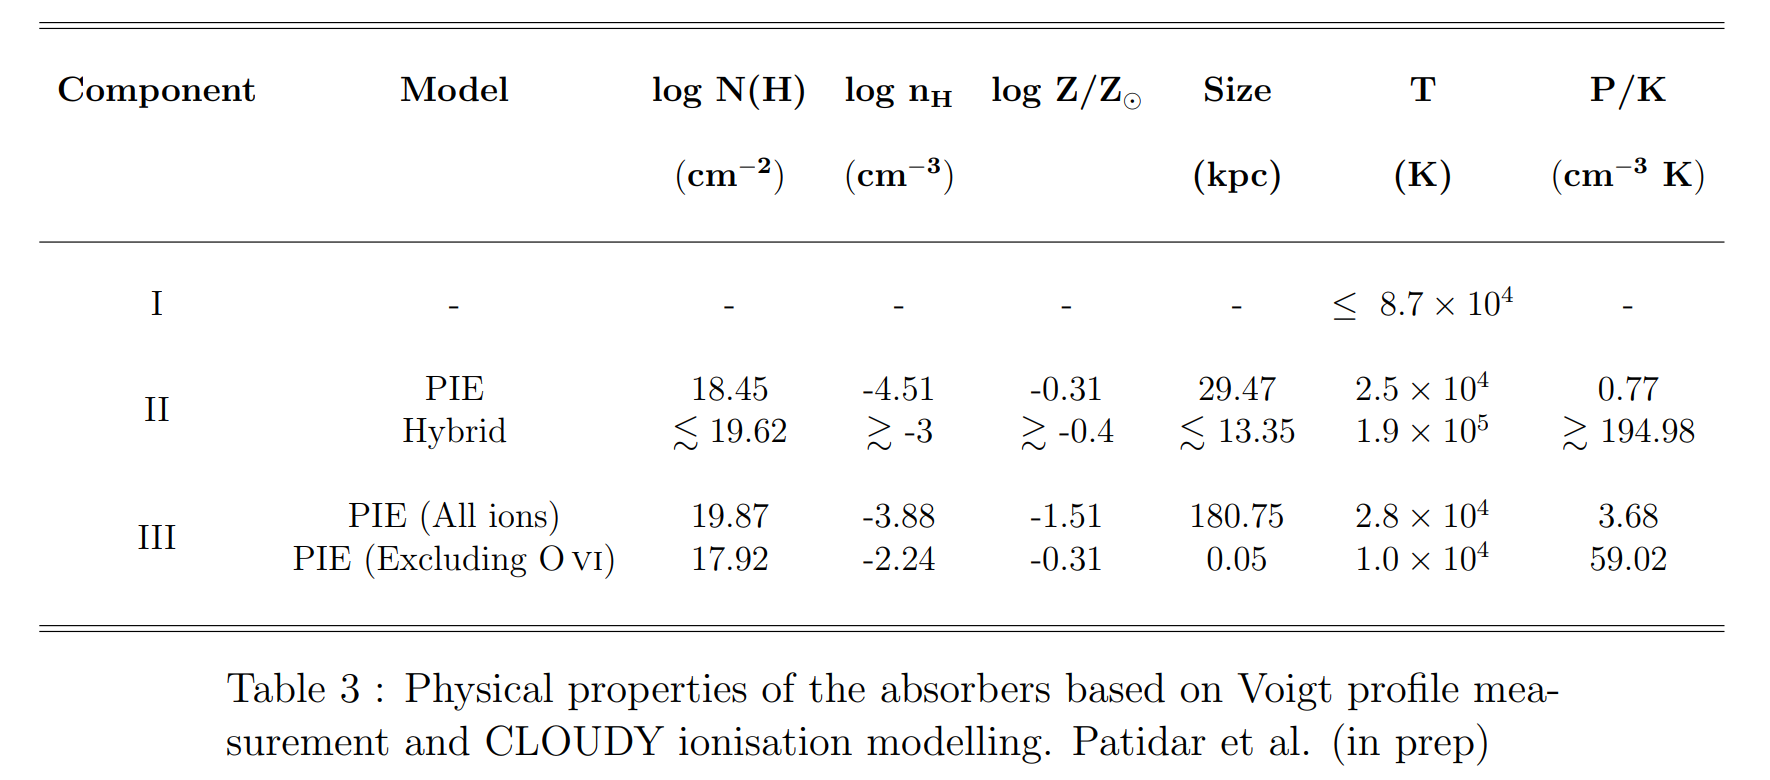
\includegraphics[width=14cm]{Figures/Mid-term/physical-params.png}
\end{figure}


\end{frame}

\section{The Survey}

\vspace*{2.7cm}

{\huge{\textbf{The Survey}}}

\end{frame}

\begin{frame}{\huge{\textbf{Hunt for BLAs}}}

\uncover<1->{
\begin{itemize}

\uncover<2->{\item Broad Ly$\alpha$ :}

$$\uncover<3->{\MyBox{b \geq 45 \ \text{km s}^{-1}}} \uncover<4->{\hspace{8mm} \Rightarrow \ \ \  \text{568 systems}}$$  

\vspace{-3mm}

\uncover<5->{\item Ionisation modelling :}
\vspace{2mm}
$$\uncover<6->{\MyBox{\text{metal ions} \geq 3}} \uncover<7->{\hspace{8mm} \Rightarrow \ \ \  \text{28 systems}}$$ 

\begin{center}
\vspace{2mm}
 \uncover<8->{\MyBox[red]{\textbf{28 BLA candidates}}}   
\end{center}

\end{itemize}
}

\end{frame}

\begin{frame}{}
    \begin{figure}[!htbp]
          \centering
          \includegraphics[width=12cm]{Figures/Mid-term/metal-ions.png}
          \vspace*{-1mm}
          \caption{No. of different metal ions in all the 28 candidate BLAs}
    \end{figure}
\end{frame}



%% ----------- References ---------- 

\begin{frame}<presentation:0>[noframenumbering]

{\cite{Fukugita-1998} \cite{Shull} \cite{cen-ostriker-1999} \cite{tepper-2013} \cite{savage-2014} \cite{danforth-2016} \cite{acharya_khaire}}
    
\end{frame}
    
% \end{frame}


\begin{frame}
\renewcommand{\bibfont}{\footnotesize}
\frametitle{\huge{\textbf{References}}}

\bibliographystyle{mnras}
\bibliography{References}

\end{frame}


% \end{markdown}

\end{document}

